%%%%%%%%%%%%%%%%%%%%%%%%%%%%% Define Article %%%%%%%%%%%%%%%%%%%%%%%%%%%%%%%%%%
\documentclass{article}
%%%%%%%%%%%%%%%%%%%%%%%%%%%%%%%%%%%%%%%%%%%%%%%%%%%%%%%%%%%%%%%%%%%%%%%%%%%%%%%

%%%%%%%%%%%%%%%%%%%%%%%%%%%%% Using Packages %%%%%%%%%%%%%%%%%%%%%%%%%%%%%%%%%%
\usepackage{graphicx}
\usepackage[margin=1in]{geometry}
\usepackage{amssymb}
\usepackage{amsmath}
\usepackage{amsthm}
\usepackage{empheq}
\usepackage{mdframed}
\usepackage{booktabs}
\usepackage{lipsum}
\usepackage{graphicx}
\usepackage{color}
\usepackage{psfrag}
\usepackage{pgfplots}
\usepackage{bm}
\usepackage{listings}
%%%%%%%%%%%%%%%%%%%%%%%%%%%%%%%%%%%%%%%%%%%%%%%%%%%%%%%%%%%%%%%%%%%%%%%%%%%%%%%

% Other Settings

%%%%%%%%%%%%%%%%%%%%%%%%%% Page Setting %%%%%%%%%%%%%%%%%%%%%%%%%%%%%%%%%%%%%%%
\geometry{a4paper}

%%%%%%%%%%%%%%%%%%%%%%%%%% Define some useful colors %%%%%%%%%%%%%%%%%%%%%%%%%%
\definecolor{ocre}{RGB}{243,102,25}
\definecolor{mygray}{RGB}{243,243,244}
\definecolor{deepGreen}{RGB}{26,111,0}
\definecolor{shallowGreen}{RGB}{235,255,255}
\definecolor{deepBlue}{RGB}{61,124,222}
\definecolor{shallowBlue}{RGB}{235,249,255}
%%%%%%%%%%%%%%%%%%%%%%%%%%%%%%%%%%%%%%%%%%%%%%%%%%%%%%%%%%%%%%%%%%%%%%%%%%%%%%%

%%%%%%%%%%%%%%%%%%%%%%%%%% Define an orangebox command %%%%%%%%%%%%%%%%%%%%%%%%
\newcommand\orangebox[1]{\fcolorbox{ocre}{mygray}{\hspace{1em}#1\hspace{1em}}}
%%%%%%%%%%%%%%%%%%%%%%%%%%%%%%%%%%%%%%%%%%%%%%%%%%%%%%%%%%%%%%%%%%%%%%%%%%%%%%%

%%%%%%%%%%%%%%%%%%%%%%%%%%%% English Environments %%%%%%%%%%%%%%%%%%%%%%%%%%%%%
\newtheoremstyle{mytheoremstyle}{3pt}{3pt}{\normalfont}{0cm}{\rmfamily\bfseries}{}{1em}{{\color{black}\thmname{#1}~\thmnumber{#2}}\thmnote{\,--\,#3}}
\newtheoremstyle{myproblemstyle}{3pt}{3pt}{\normalfont}{0cm}{\rmfamily\bfseries}{}{1em}{{\color{black}\thmname{#1}~\thmnumber{#2}}\thmnote{\,--\,#3}}
\theoremstyle{mytheoremstyle}
\newmdtheoremenv[linewidth=1pt,backgroundcolor=shallowGreen,linecolor=deepGreen,leftmargin=0pt,innerleftmargin=20pt,innerrightmargin=20pt,]{theorem}{Theorem}[section]
\theoremstyle{mytheoremstyle}
\newmdtheoremenv[linewidth=1pt,backgroundcolor=shallowBlue,linecolor=deepBlue,leftmargin=0pt,innerleftmargin=20pt,innerrightmargin=20pt,]{definition}{Definition}[section]
\theoremstyle{myproblemstyle}
\newmdtheoremenv[linecolor=black,leftmargin=0pt,innerleftmargin=10pt,innerrightmargin=10pt,]{problem}{Problem}[section]
%%%%%%%%%%%%%%%%%%%%%%%%%%%%%%%%%%%%%%%%%%%%%%%%%%%%%%%%%%%%%%%%%%%%%%%%%%%%%%%

%%%%%%%%%%%%%%%%%%%%%%%%%%%%%%% Plotting Settings %%%%%%%%%%%%%%%%%%%%%%%%%%%%%
\usepgfplotslibrary{colorbrewer}
\pgfplotsset{width=8cm,compat=1.9}
%%%%%%%%%%%%%%%%%%%%%%%%%%%%%%%%%%%%%%%%%%%%%%%%%%%%%%%%%%%%%%%%%%%%%%%%%%%%%%%

%%%%%%%%%%%%%%%%%%%%%%%%%%%%%%% Title & Author %%%%%%%%%%%%%%%%%%%%%%%%%%%%%%%%
\title{\textbf{BANA 620 PROJECT REPORT: DESCRIPTIVE AND PREDICTIVE ANALYTICS APPLIED TO THE SKILLED NURSING FACILITY COST REPORTS}}
\author{Joshua Cabal \\ \\ \\California State University, Northridge \\}
%%%%%%%%%%%%%%%%%%%%%%%%%%%%%%%%%%%%%%%%%%%%%%%%%%%%%%%%%%%%%%%%%%%%%%%%%%%%%%%

\begin{document}
    \maketitle
    \pagebreak
    \tableofcontents    
    \newpage


%-------------------BEGIN: Executive Summary------------------------------------
\section{Executive Summary}

An overview of the project, including key findings, recommendations, and a brief summary of the analysis conducted. This section should be concise and geared toward readers who may not delve into the full details of the report. 

%-------------------END: Executive Summary------------------------------------
%-------------------BEGIN: Introduction------------------------------------
\section{Introduction}

Context and background information about the opportunity the project addresses. This section should outline the objectives of the project and the significance of the analysis being conducted.
%-------------------END: Introduction------------------------------------
%-------------------BEGIN: Methodology------------------------------------
\section{Methodology}
A detailed description of the analytical methods and tools used in the project. This should include data collection processes, data analysis techniques (e.g., statistical methods, machine learning algorithms), and any software or programming languages utilized.



%-------------------END: Methodology------------------------------------
%-------------------BEGIN: Data Description------------------------------------
\section{Data Description}

An overview of the data set(s) used, including sources, size, and characteristics of the data. Highlight any data cleaning or preprocessing steps undertaken to prepare the data for analysis.



\subsection{Skilled Nusing Facility Cost Report}


Medicare-certified institutional providers are required to submit annual cost reports. These data files contain the highest level of cost report status for cost reports in each reported fiscal years. The cost report contains provider information such as facility characteristics, utilization data, cost and charges by cost center (in total and for Medicare), Medicare settlement data, and financial statement data. CMS maintains the cost report data in the Healthcare Provider Cost Reporting Information System (HCRIS). Skilled Nursing Facilities (SNF) submit their cost report data to HCRIS using form CMS-2540-2010. The reports used are from the years 2015 through 2021.

\subsubsection{Preprocessing}








%-------------------END: Data Description------------------------------------
%-------------------BEGIN: Analysis and Findings------------------------------------
\section{Analysis and Findings}

Presentation of the analysis conducted, including data visualization (charts, graphs, tables) and statistical outputs. This section should detail the insights gained from the analysis, interpreting the results in the context of the business problem.
%-------------------END: Analysis and Findings------------------------------------
%-------------------BEGIN: Discussion------------------------------------
\section{Discussion}
Interpretation of the findings, discussing how they address the project objectives and their implications for the business. This section should also cover any limitations of the analysis and considerations for future research.

%-------------------END: Discussion------------------------------------
%-------------------BEGIN: Recommendations------------------------------------
\section{Recommendations}
Based on the analysis and findings, provide actionable recommendations for the business. Clearly articulate the expected impact of these recommendations and suggest a plan for implementation.

%-------------------END: Recommendations------------------------------------
%-------------------BEGIN: Conclusion------------------------------------
\section{Conclusion}
Summarize the key points from the report, reinforcing the value of the findings and recommendations.

%-------------------END: Conclusion------------------------------------
%-------------------BEGIN: Appendices------------------------------------
\section{Appendices}
Include any additional material that supports the analysis, such as detailed data tables, code snippets, or extended methodology descriptions.

\begin{figure}[htbp]
\centering
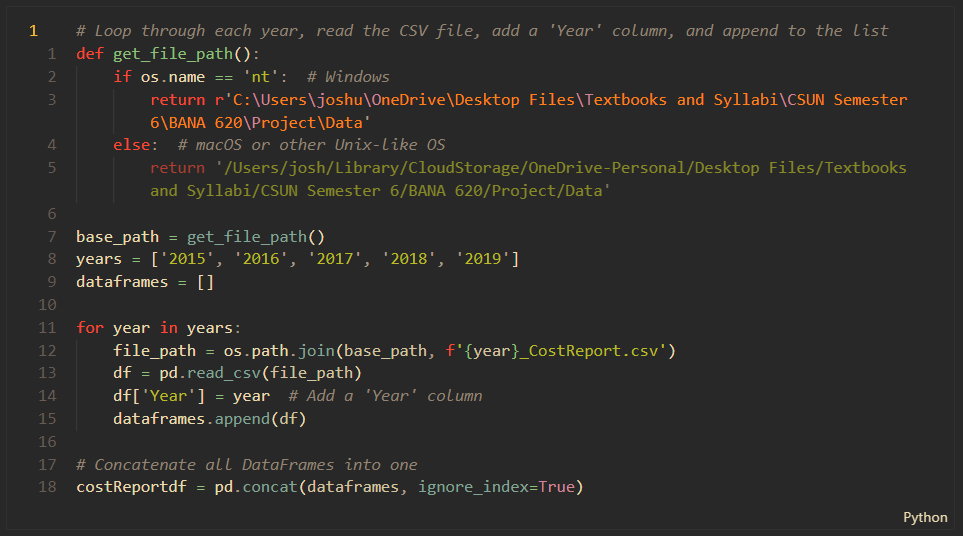
\includegraphics[width=\linewidth]{./Images/dataLoadingSnippet.png}
\caption{Data loading code snippet}
\label{fig:screenshot_label}
\end{figure}

%-------------------END: Appendices------------------------------------

%-------------------BEGIN: References------------------------------------
\section{References}
List all sources cited in the report, including data sources, literature, and any external references used in the analysis.

%-------------------END: References------------------------------------



\end{document}